% vim: set spelllang=fr:

\setchapterpreamble[ur][.6\textwidth]{%
  \dictum[Bill Watterson, \textit{Calvin et Hobbes}]{%
    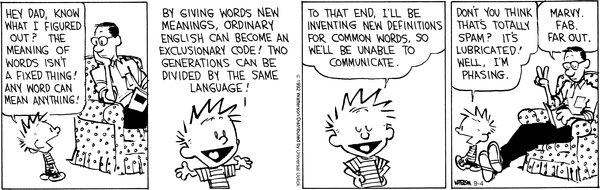
\includegraphics[width=0.6\textwidth]{fig/calvin_meaning.png}}}

\chapter{Annotation en rôle sémantique en domaine spécifique}
\label{ch:domainsrl}

% TODO  ?
% Evaluating our approach on domain-specific corpora such as the Kicktionary
% \citep{schmidt2009kicktionary}, the Robocup dataset \citep{chen2008learning} or
% the Situated Language dataset \citep{bordes2010towards} and compare our method
% with existing domain-specific semantic role labeling work
% \citep{wyner2010lexical,hadouche2011annotation,goldwasser2013leveraging}.

We present a free software baseline for Semantic Role Labeling that only uses
VerbNet to assign roles to arguments in a sentence. The approach is
domain-independent and easily reproducible as it simply matches verb arguments
to VerbNet frames which is designed to cover general text.  Our system is
therefore suitable either as a strong baseline, a first step towards annotating
a new domain or a full Semantic Role Labeling system once VerbNet has been
slightly updated towards the new domain. Additionally, it can be used to
highlight gaps in VerbNet that have remained unnoticed until now.

\section{Introduction}

Semantic Role Labeling on new domains is still an open problem.  Existing
approaches either require some annotated data or transfer a model from a
related domain. We propose an approach where no domain-specific data is needed
as we only use the VerbNet lexical resource. As a result, this approach is
simple, does not require an annotated corpus and is easily adaptable to
languages with a VerbNet-like resource such as Estonian
\citep{jentson2014verbnet}, French \citep{pradet2014adapting} or Portuguese
\citep{scarton2012towards}.

Là où le précédent chapitre présentait sur l'annotation en rôles sémantiques
fondée sur la connaissance, celui-là se concentre sur l'annotation en domaines
spécifiques.

La définition du terme 'domaine' reste assez vague dans le sens où il est
difficile de proposer une catégorisation de la connaissance en un ensemble de
domaines qui soit à la fois cohérente et efficace pour le Traitement Automatique
des Langues. Il est aussi difficile de séparer clairement le «~domaine
général~» des domaines spécifiques.

% TODO wordnet domains issues ma2012rethinking

Néanmoins, c'est un phénomène qui existe et qui est à considérer : les modèles
entraînés sur un corpus d'un domaine spécifique (la finance par exemple)
généraliseront mal à d'autres domaines (le football) par exemple. % proof

À l'heure où les algorithmes supervisés obtiennent d'excellentes performances
sur un certain nombre de tâche, l'adaptation au domaine est un défi majeur du
Traitement Automatique des Langues.

Il est important aussi de différencier le genre et le domaine d'un texte. Le
corpus du Wall Street Journal traite du domaine de la finance dans un genre
journalistique. D'autres genres existent, par exemple les genre littéraires que
sont la fiction, la poésie, le théâtre, etc. Néanmoins, ces distinctions ne
nous concernent pas ici, et l'objectif affiché est de traiter aussi bien un
roman qu'une encyclopédie qu'un email bien écrit qu'un article de journal.
C'est une simplification mais les difficultés que nous rencontrons avec les
corpus utilisés dépendent plutôt du domaine que du genre. En effet, dans deux
domaines différents plus que dans deux genres différents, les changements vont
résider dans les verbes utilisés, leur sens et la façon de les utiliser. C'est
ce que nous souhaitons prendre en compte ici.


\section{Prior work}

SEMAFOR \citep{das2014frame} is the supervised system closest to our approach.
Using the FrameNet corpus, it first identifies predicates, then identify the
correct frame evoked by those predicates, and finally performs argument
identification by detecting which word spans in a sentence carry a role for the
identified predicate.

We leave the span identification part of argument identification to future
work, considering the gold argument spans: the goal is to determine the role of
each span. The reason is that we currently want to focus on the ability of
VerbNet to annotate FrameNet-style domain-specific corpora.

\cite{chen2008learning} train a commentator system using
existing commentaries and simulation states of soccer games, but without
explicit knowledge about the English language. Their approach spurred work on
situated language understanding: \cite{bordes2010towards}
and \cite{richardson2012towards} later proposed other
corpora for situated language understanding systems. Our system is similar in
that we minimize human effort to automatically annotate new domains, but we
focus on FrameNet-style Semantic Role Labeling rather than situated language
understanding.

The Semantic Role Labeling system of \cite{gormley2014low} does not need
supervised syntax, but still requires a role-labelled corpus.
\cite{hadouche2011annotation} performs Semantic Role Labeling on one of our
three corpora (DiCoInfo) with two approaches: (i) applying manually crafted
rules to the output of a syntactic parser (ii) learning a supervised system
with various features from the literature. They highlight the need of
annotating more examples to get better results on a wider range of roles and
predicates. Our work goes the opposite direction: we show that by using less
supervised data, it is possible to annotate a large number of sentences from
various domains.

\section{Approach}

\subsection{VerbNet}
\label{subsec:verbnet}

\cite{levin1993english} argues that syntactic alternations reflect the
underlying semantics of verb senses. Observing those alternations allows to
create semantic classes, grouping together verb senses sharing roughly the same
semantics and the same thematic roles. The resulting resource has since been
digitized and expanded with new verb classes, new complements, new lemmas and
new syntactic frames, producing VerbNet \cite{kipperschuler2005verbnet}.

Due to the way it was built, VerbNet is a natural fit for Semantic Role
Labeling as it provides an explicit syntax-semantics interface that allows to
tag verb subjects and objects with semantic roles. It also has the additional
benefit to cover 6000 verb senses. It is far from WordNet's 13000 verb synsets,
and still needs to be improved, but it already contains enough lemmas for many
use cases, as we show in section~\ref{sec:domainsrlresults}.

For a given class such as \texttt{put-9.1}, VerbNet lists verbs, semantic roles
and VerbNet frames\footnote{A FrameNet frame corresponds to a VerbNet class,
while a VerbNet frame describes a subcategorization frame.}, that we will note
as follows: \texttt{NP.Agent} \texttt{V} \texttt{\{\{+loc\}\}}
\texttt{NP.Theme} \texttt{PP.Destination}. In this case, the subject of the
verb is \texttt{Agent}, the first object is \texttt{Goal} and the second one is
\texttt{Theme}. Here, roles are filled by two noun phrases and a prepositional phrase
introduced with a preposition of location, but other complements are present in
VerbNet. In addition to this information, frames come with an example (eg.
\textit{I put the book on the table}) and semantics expressed using first-order
logic that we ignore in this work.

\subsection{Algorithm}

To annotate a given sentence with already identified role fillers, we first
list all the classes that can be triggered by a given verb. For example, given
the sentence \emph{The online judge allocates the same amount of memory to both
chess engines}, the only possible class for verb \emph{allocate} is
\texttt{future\_having-13.3}. In other cases, the choice could be ambiguous,
eg. for \emph{The ocean circulation transports warm water to the North Atlantic}
where the \texttt{amuse-31.1} and \texttt{send-11.1} classes both contain the
\textit{transport} verb.

Now that a list of classes has been established, the sentence is represented
using VerbNet notation, which is \texttt{NP} \texttt{V} \texttt{NP}
\texttt{\{to\}} \texttt{PP} for our two example sentences.

Next, simple transformations account for specific ways to encode frames in
DiCoInfo and DiCoEnviro. First, repeating roles are removed: \texttt{NP.Agent}
\texttt{V} \texttt{NP.Theme} \texttt{NP.Theme} is transformed to
\texttt{NP.Agent} \texttt{V} \texttt{NP.Theme}, as syntactic frames do not
duplicate roles, while DiCoInfo and DiCoEnviro do when two noun phrases linked
with 'and' occur. Second, when encountering \texttt{V} \texttt{NP.Theme}, the
role before the verbs are also removed in VerbNet frames before comparison.

This transformed sentence frame is then compared to possible VerbNet frames in
the candidate classes. For the first sentence, the only possible option is
\texttt{NP.Agent} \texttt{V} \texttt{NP.Theme} \texttt{\{to\}} \texttt{PP.Goal}
(\textit{We offered our paycheck to her}) from the \texttt{future\_having-13.3}
class. For the second sentence, the only possible option is \texttt{NP.Agent}
\texttt{V} \texttt{NP.Theme} \texttt{\{to\}} \texttt{PP.Destination} in the
\texttt{send-11.1} class. Considering the subcategorization frames allowed to
identify the correct class and to assign semantic roles to frame elements.

Two difficulties can arise when performing this frame matching:
\begin{itemize}
    \item the frame is not present in any candidate VerbNet class: VerbNet lacks this frame.
    \item the frame does not allow to disambiguate between different classes and different roles.
\end{itemize}

While our approach is too simple to deal with the second difficulty, the first
one highlights missing information in VerbNet. The result of this algorithm is
that every predicate is possible associated with a VerbNet class, and every
gold role filler is possibly assigned to a semantic role.\footnote{The source
code of this experiment is available at \url{http://anonymized}}.

\section{Enrichissement de VerbNet}

Malgré leur similarité, ces corpus posent des problèmes différents vis-à-vis de
leur annotation avec VerbNet, tous liés au fait de ne pas être dans le "domaine
général". Nous avons considéré comme problème les manquements dans VerbNet qui
empêchent de prendre en compte les phrases considérées, indépendamment de
l'algorithme. Ainsi, pour que VerbNet puisse prendre en compte une instance, il
faut :

\begin{itemize}
    \item que le sens du verbe considéré soit présent dans VerbNet,
    \item que la construction en question soit présente dans VerbNet,
    \item et que les rôles sémantiques associés à chaque syntagme soient correct.
\end{itemize}

Il y a différentes façons de ne pas respecter ces contraintes :

\begin{itemize}
    \item Le verbe n'existe pas du tout dans VerbNet
    \item Le sens du verbe utilisé n'est pas représenté dans VerbNet alors que c'est un sens du domaine général
    \item Le sens du verbe utilisé n'est pas représenté dans VerbNet alors que c'est un sens spécifique à ce domaine
    \item La construction utilisée n'est pas présente dans VerbNet
    \item La construction utilisée est incorrecte dans VerbNet
\end{itemize}

Suivant les corpus considérés, les proportions d'erreurs seront différentes.
Nous avons demandé à deux annotateurs d'évaluer, pour vingt phrases par
domaine, quelle était l'erreur. L'accord inter-annotateur permet de valider la
distinction domaine spécifique/domaine général malgré l'impossibilité de la
définir précisément. % TODO lefaire

C'est pour cette raison que l'enrichissement de VerbNet se fait de deux
manières : certains verbes et constructions sont ajoutés comme faisant partie
du domaine général, alors que d'autres sont étiquetés avec le domaine
spécifique correspondant. L'idée est d'éviter que des connaissances de domaines
spécifiques viennent réduire la qualité de la ressource tout en s'assurant que
la couverture de VerbNet pour le domaine général continue de s'améliorer.

\subsection{Détection semi-automatique d'erreurs}

D'une part, pour minimiser le travail manuel, il est important d'automatiser au
maximum l'enrichissement de la ressource. D'autre part, l'intérêt de VerbNet
réside notamment dans sa capacité à factoriser efficacement ces informations
sur l'interface syntaxico-sémantique d'un verbe donné, et il est donc possible
et utile de valider manuellement chacun des changements apportés.

Le principe suivi est donc d'essayer de détecter les manquements de VerbNet de
manière automatique avant de proposer à un utilisateur expert de réaliser des
changements en ayant un maximum d'informations pertinentes à portée de main.

Les différentes erreurs détectées sont :
\begin{itemize}
    \item l'absence de lemmes dans la ressource
    \item l'absence d'un sens correct dans la ressource
    \item l'absence de constructions correctes dans la ressource
    \item l'absence de mapping de role correct dans la ressource
\end{itemize}

Nous avons d'abord commencé par détecter l'absence de constructions correctes,
ce qui a permis ensuite de détecter une absence de sens en comparant les
constructions observées avec les constructions présentes. Enfin, cela a permis
de faire des propositions quant à la position d'un nouveau lexème dans la
ressource.

\section{Experiments}


\subsection{Corpus considérés}

Afin de s'assurer que notre travail reste valide en changeant de domaine, nous
considérons ici trois corpus présents dans des domaines différents :

\begin{itemize}
    \item le Kicktionary rassemblant des dépêches de l'UEFA dans le domaine du football,
    \item DicoInfo~: corpus Informatique/Internet de l'OLST,
    \item et DicoEnviro~: le corpus Réchauffement climatique de l'OLST
\end{itemize}

Les points communs majeurs de ces trois corpus sont :
\begin{enumerate}
    \item de s'inspirer librement de la théorie des Frame Semantics telle qu'elle est considérée dans FrameNet,
    \item d'être disponible à la fois en anglais et en français,
    \item d'être basés sur l'annotation dans un corpus d'un certain nombre de prédicats (ce n'est pas une annotation dite "full-text")
\end{enumerate}

Ce dernier point est plutôt un inconvénient : la manière la plus réaliste de
considérer un corpus d'entraînement est de réaliser une annotation dite
\textit{full-text} en annotant tous les prédicats rencontrés dans un texte
donné. Cependant, les contextes choisis dans DicoInfo et DicoEnviro l'ont été
sur des critères de diversité syntaxique. \citep{lhomme2012adding} Le postulat
que nous faisons dans ce travail est que notre méthode n'est pas affectée par
ce problème comme le serait un modèle statistique appris sur ces mêmes
contextes étant donné que la probabilité des différentes possibilités n'est pas
prise en compte.
To compare the results across domains, we consider three domain-specific
frame-annotated corpora.

\begin{itemize}

\item The Kicktionary soccer corpus \cite{schmidt2009kicktionary} contains
sentences of UEFA reports about the Europa League, the Champions League and the
World Cup. It is available in English, French and German.

\item the DiCoInfo corpus\footnote{\label{olst}Corpus spécialisés de
l'Observatoire de linguistique Sens-Texte (OLST).} contains sentences from the
domains of computing and the Internet in English, French and Spanish.

\item the DiCoEnviro\cite{corpusolst} corpus contains sentences from the
environment domain (mainly climate change) in English, French and Spanish.

\end{itemize}

We chose those three corpora because they were annotated with the FrameNet
methodology in mind, which is a good fit for VerbNet while being more
semantically precise than PropBank. Kicktionary lexical units include verbs,
nouns, adjectives and idiomatic expressions. The DiCoInfo and DiCoEnviro also
contain multiple parts of speech but currently focus on verbs.  We only
consider verbs in this work.

All three corpora were split in half with a ``training'' set and a test set.
Since there is no model to be trained, the ``training'' set is only used to
understand the errors in our algorithm and in VerbNet. While all three corpora
contain related texts, they come from different sources and were written by
different authors. We normalized those sources (eg. DEBIAN2 and DEBIAN3 become
DEBIAN) and used this information when splitting the corpora: a specific source
can only be present in one of the two sets.\footnote{The resulting split is
available online for reproduction purposes at \url{http://anonymized}.}

\subsection{Role mappings}

All three corpora use specific roles. The DiCoInfo and DiCoEnviro use VerbNet
conventions while the Kicktionary, following FrameNet more closely, defines a
new set of roles for each frame, such as \texttt{Passer}, \texttt{Moving\_Ball}
or \texttt{Shot}. We therefore needed to establish a mapping between VerbNet
roles and DiCoInfo, DiCoEnviro and Kicktionary roles. We manually assigned a
VerbNet class to every domain frame.\footnote{The resulting mappings are
available online at \url{http://anonymized}.}

DiCoInfo and DiCoEnviro distinguish between core and non-core roles: we only
annotated core roles as they correspond to VerbNet roles which ignores adjuncts
as they don't allow to separate verb senses. Since a DiCoInfo/DiCoEnviro frame
is a specific verb sense accepting specific alternations, we always mapped them
to a single VerbNet class.

The Kicktionary corpus proved more difficult to map to VerbNet than the other
two as frames in the Kicktionary sometimes include a large number of different
verbs behaving differently. FrameNet frame development rules specify that such
frames should have been split \cite{ruppenhofer2006extended}, but the
Kicktionary doesn't always follow those rules. Some frames are correctly
defined, such as \texttt{Receive\_Card} and \texttt{Give\_Card} who
respectively map to \texttt{obtain-13.5.2} and \texttt{give-13.1-1}. However,
for example, the \texttt{Goal} frame appears to be defined as scoring a goal,
but the various way to express this are not separated: open the scoring,
equalise, strike, score, etc. will use different syntactic alternations, evoke
different roles and map to different VerbNet classes. The mapping of those
frames is still ongoing, which explains that Kicktionary results for class
accuracy are currently lower than those of DiCoInfo and DiCoEnviro.

\section{Méthode d'évaluation}

Les trois corpus considérés ont été annotés en rôles sémantiques dans les deux
langues qui nous intéressent ici~: l'anglais et le français. Il nous suffit
donc d'utiliser un mapping entre les rôles considérés par ces ressources et les
rôles VerbNet avant d'évaluer la performance de l'algorithme basé sur la
connaissance d'annotation en rôles sémantiques présenté au
chapitre~\ref{ch:srl}.

Dans le cas de DicoInfo et DicoEnviro, les noms des rôles sont proches des noms
de rôles employée dans VerbNet et LIRICS \citep{bonial2011hierarchical} (Agent,
Patient, Destination, Instrument...). Cependant, même si les noms sont les
mêmes, la définition de ces rôles est spécifique à DicoInfo et DicoEnviro.
En pratique :

\begin{itemize}
    \item DicoInfo et DicoEnviro ne distinguent pas Theme de Patient mais
    n'utilise que Patient ce qui rend l'annotation plus facile.\footnote{La
    distinction entre Theme et Patient est difficile à établir. Dans \textit{Le
    chaton a léché mes doigts}, est-ce que mes doigts ont changé d'état ? Si oui,
    ils devraient être Patient, et sinon, Theme.\citep[p.~5]{palmer2010semantic}}
    \item Pour un certain nombre de lexies, la perspective du domaine implique
    souvent des rôles différents (TODO exemple Patient vs. Result) % TODO clair
\end{itemize}

C'est pour ces raisons que nous avons créé manuellement un mapping entre
VerbNet et les corpus considérés (DicoInfo et DicoEnviro). Ce mapping est
utilisé uniquement à des fins d'évaluation, et l'effort nécessaire pour le
créer n'est donc pas à prendre en compte pour calculer l'effort global
nécessaire pour notre approche. Prenons deux phrases d'exemple pour illustrer
le mapping. Voici deux phrases présentes dans DicoInfo et DicoEnviro :

\begin{itemize}
    \item In the interest of fair competition you should ALLOCATE the same amount of memory to both engines.
    \item Techniques and tools exist to MEASURE carbon stocks in project areas relatively precisely depending on the carbon pool.
\end{itemize}

Dans la première phrase, le sens du verbe \textit{allocate} est très précis et
très spécifique au domaine de l'informatique. Pourtant, il se comporte
syntaxiquement de la même manière que le sens plus général considéré par
WordNet et OntoNotes: \textit{distribute or se aside according to plan}. Par
conséquent, un mapping manuel a été réalisé de la lexie allocate.1 (qui
correspond à la phrase ci-dessus) vers la classe Verbnet
\textit{future\_having-13.3}. Enfin, les actants définis par DicoInfo (qui
correspondent aux roles \textit{Core} de FrameNet et aux rôles de VerbNet) ont
étés mis en correspondance avec les rôles de VerbNet :

\begin{itemize}
    \item Patient devient Theme
    \item Recipient devient Goal
    \item Agent reste Agent
\end{itemize}

Une fois que ce mapping est réalisé, la tâche de notre algorithme d'annotation
en rôles sémantiques devient de détecter que la classe future\_having-13.3 est
utilisée ici, que 'You' est Agent, que 'the same amount of memory' est Theme,
et que 'to both engines' est Goal. La démarche est la même pour la seconde
phrase, où il s'agit d'identifier que \textit{Techniques and tools} est Agent,
et que \textit{carbon stocks} est Theme.


\section{Results}
\label{sec:domainsrlresults}

We first consider VerbNet's coverage of those three resources, measuring lemma
coverage, syntactic coverage, and role coverage. Each of those is computed
considering tokens, not types.

\begin{table}[h]
\centering
\begin{tabular}{rccc}
  \toprule
        & Info & Enviro & Kicktionary \\
  \midrule
  Lemma & 83 & 84 & 75 \\
  Frame & 79 & 78 & 67 \\
  Class & 51 & 64 & 6  \\
  Role  & 91 & 97 & 70 \\
  \bottomrule
\end{tabular}

\caption{\protect\label{table:coverage} VerbNet coverage for the DiCoInfo,
DiCoEnviro and Kicktionary resources. Lemma is the percentage of verb lemma
tokens that are present in VerbNet. Frame is the percentage of exact frame
matches between VerbNet and the domain-specific corpora when the lemma was in
VerbNet. Class is the percentage of classes that were correctly identified
according to our mapping when the frame was in VerbNet. Finally, Role is the
percentage of correctly identified roles when the class has been correctly
identified.}

\end{table}

Table~\ref{table:coverage} shows the results for the three considered domains.
The Kicktionary results should be considered carefully as the reasons for
errors were not fully analyzed yet. Some conclusions can still be drawn from
the current results. First, VerbNet covers between 75\% and 84\% of lemma
tokens for unseen domain corpora, highlighting the promising coverage of
VerbNet.  Second, while the results vary between domains, those results are
still preliminary and the results can change depending on the way frames are
encoded (the training set of the Kicktionary corpus has not been analyzed yet).
Still, based on lemma coverage, the Kicktionary corpus seems to be the farthest
from VerbNet. Third, once the class has been correctly identified, the results
are good in the DiCoInfo and DiCoEnviro corpora.

Note that missing verbs are not necessarily domain-specific, and considering
those three domains highlights coverage gaps in VerbNet that were not
necessarily apparent when using the PropBank and FrameNet corpora. One example
of a missing lemma in the Kicktionary is \textit{celebrate}: while frequent in
sports corpora, it would still be useful in general domain text.

\section{Conclusions}

We showed that it is possible to perform Semantic Role Labeling using VerbNet.
The actual Semantic Role Labeling will be implemented as future work, reusing
the simple frame-matching approach of \cite{swier2005exploiting} for
domain-specific corpora.

Our current approach can be used to begin annotating a new domain before
switching to manual annotation. It is also possible to use it as a simple
baseline for more sophisticated domain Semantic Role Labeling approaches.
Finally, annotating new domains is a good way to guide new VerbNet developments
as it shows missing lemmas, classes and frames.

\section*{Acknowledgments}

We would like to thank Thomas Schmidt and Marie-Claude L'Homme for providing
us the Kicktionary, DiCoInfo and DiCoEnviro corpora.
